\documentclass[12pt]{article}
% Paper size: A4 (8.27in x 11.69in / 210mm x 297mm)
\usepackage[paperwidth=8.27in,paperheight=11.69in,margin=0in]{geometry}
\usepackage{tikz}
\usepackage{helvet}
\renewcommand{\familydefault}{\sfdefault}
\pagestyle{empty}

% Mini-sheet Parameters (Inches)
\newcommand{\numQuestions}{50}       % 50 Items Default
\newcommand{\numChoices}{4}          % A, B, C, D
\newcommand{\rowsPerCol}{25}         % 25 rows per column (Col 1: Q1-25, Col 2: Q26-50)
\newcommand{\colOffset}{1.80}        % Horizontal distance between columns (in)

\newcommand{\startX}{0.35}          
\newcommand{\startY}{1.15}          
\newcommand{\stepX}{0.20}
\newcommand{\stepY}{0.16}          
\newcommand{\bubbleRadius}{0.055}
\newcommand{\markerSize}{0.10}
\newcommand{\markerMargin}{0.15}

\def\choiceLetters{A,B,C,D}

\begin{document}

\begin{tikzpicture}[remember picture, overlay, x=1in, y=-1in, shift={(current page.north west)}]

  % Tile 4 mini sheets: 2 columns (X) x 2 rows (Y)
  \foreach \gridX in {0, 1} {
    \foreach \gridY in {0, 1} {
      
      % Calculate Top-Left Origin of each quarter sheet (4.135in x 5.845in)
      \pgfmathsetmacro{\offsetX}{\gridX * 4.135}
      \pgfmathsetmacro{\offsetY}{\gridY * 5.845}

      % 1. Cutting Guide Lines
      \draw[gray, dashed, line width=0.3pt] 
        (\offsetX, \offsetY) rectangle (\offsetX + 4.135, \offsetY + 5.845);

      % 2. Corner Fiducial Markers
      \pgfmathsetmacro{\leftX}{\markerMargin}
      \pgfmathsetmacro{\rightX}{4.135 - \markerMargin}
      \pgfmathsetmacro{\topY}{\markerMargin}
      \pgfmathsetmacro{\bottomY}{5.845 - \markerMargin}

      \foreach \cx/\cy in {\leftX/\topY, \rightX/\topY, \leftX/\bottomY, \rightX/\bottomY} {
        \fill[black] (\offsetX + \cx - \markerSize/2, \offsetY + \cy - \markerSize/2)
                     rectangle (\offsetX + \cx + \markerSize/2, \offsetY + \cy + \markerSize/2);
      }

      % 3. Header Block
      \node[anchor=north west, font=\bfseries\small] at (\offsetX + \markerMargin + 0.1, \offsetY + \markerMargin + 0.02) {OMR Answer Sheet (50 Qs)};
      \node[anchor=north west, font=\tiny] at (\offsetX + \markerMargin + 0.1, \offsetY + \markerMargin + 0.35) {Name: \underline{\hspace{1.5in}} \quad Sec/ID: \underline{\hspace{0.7in}}};

      % 4. 50-Item Bubble Grid (2 Columns of 25)
      \foreach \q in {1,...,\numQuestions} {
        % Calculate column (0 or 1) and row index (0 to 24)
        \pgfmathtruncatemacro{\colIndex}{(\q-1)/\rowsPerCol}
        \pgfmathtruncatemacro{\rowIndex}{mod(\q-1,\rowsPerCol)}

        \pgfmathsetmacro{\rowY}{\offsetY + \startY + \rowIndex*\stepY}
        \pgfmathsetmacro{\baseX}{\offsetX + \startX + \colIndex*\colOffset}

        % Question Number Label
        \node[anchor=east, font=\tiny] at (\baseX - 0.08, \rowY) {\q.};

        % Answer Choices
        \foreach \c [count=\ci from 0] in \choiceLetters {
          \ifnum\ci<\numChoices
            \pgfmathsetmacro{\colX}{\baseX + \ci*\stepX}
            \draw[black, line width=0.4pt] (\colX, \rowY) circle (\bubbleRadius);
            \node[font=\fontsize{3.5}{3.5}\selectfont] at (\colX, \rowY) {\c};
          \fi
        }
      }

    }
  }

\end{tikzpicture}

\end{document}
